\documentclass[11pt,a4paper]{article}
\usepackage[utf8]{inputenc}
\usepackage[T1]{fontenc}
\usepackage[french]{babel}
\usepackage{geometry}
\usepackage{graphicx}
\usepackage{listings}
\usepackage{xcolor}
\usepackage{hyperref}
\usepackage{booktabs}
\usepackage{array}
\usepackage{longtable}
\usepackage{amssymb}

\geometry{margin=2.5cm}

\lstset{
  basicstyle=\ttfamily\small,
  keywordstyle=\color{blue},
  commentstyle=\color{gray},
  stringstyle=\color{orange},
  breaklines=true,
  frame=single
}

\newcommand{\ok}{\textcolor{green!60!black}{\textbf{true}}}
\newcommand{\ko}{\textcolor{red!70!black}{\textbf{false}}}
\newcommand{\err}[1]{\textcolor{purple}{\textbf{throw} \small\textit{#1}}}

\title{T2112 --- Devoir 2 \\[0.4em]\large Qualité logicielle : Catalog-Based Testing, Pairwise \& Code Coverage}
\author{Nom : KETELS Noah}
\date{Mars 2026}

\begin{document}
\maketitle
\tableofcontents
\bigskip

% =========================================================
\section{Introduction}
% =========================================================

Ce rapport présente la démarche complète appliquée pour tester et valider la fonction
\texttt{validateUserRegistration(age, role, email)}, une nouvelle fonctionnalité de l'API
chargée de vérifier les données d'un nouvel utilisateur avant son enregistrement en base de données.

La démarche suit trois étapes ordonnées :
\begin{enumerate}
  \item \textbf{Black Box Testing} --- identification des valeurs limites et des cas d'erreur
        par la méthode du \emph{Catalog-Based Testing}, puis réduction des combinaisons via le
        principe \emph{Pairwise}.
  \item \textbf{Implémentation} --- codage de la fonction en TypeScript dans
        \texttt{src/utils/userValidator.ts}.
  \item \textbf{White Box Testing} --- rédaction de la suite de tests dans
        \texttt{src/tests/userValidator.test.ts} avec l'objectif d'atteindre
        \textbf{100\% de Branch Coverage}.
\end{enumerate}

% =========================================================
\section{Black Box Testing --- Catalog-Based Testing}
% =========================================================

\subsection{Identification des classes d'équivalence et valeurs limites}

\paragraph{Paramètre \texttt{age} (number)}
\begin{itemize}
  \item \textbf{Valeur invalide au-delà de la borne supérieure :} $age > 120$
        $\Rightarrow$ \texttt{throw new Error("Âge invalide")}
  \item \textbf{Borne supérieure maximale valide :} $age = 120$ $\Rightarrow$ continuer le traitement
  \item \textbf{Partition adulte :} $18 \leq age \leq 120$ $\Rightarrow$ valide, traitement email
  \item \textbf{Borne inférieure adulte :} $age = 18$ $\Rightarrow$ valide (limite basse adulte)
  \item \textbf{Mineur limite haute :} $age = 17$ $\Rightarrow$ inscription refusée (sauf stagiaire)
  \item \textbf{Partition mineur :} $age < 18$ $\Rightarrow$ refus sauf si rôle = "stagiaire"
\end{itemize}

\paragraph{Paramètre \texttt{role} (string)}
\begin{itemize}
  \item \textbf{Valeur valide 1 :} \texttt{"admin"} $\Rightarrow$ accepté
  \item \textbf{Valeur valide 2 :} \texttt{"user"} $\Rightarrow$ accepté
  \item \textbf{Valeur valide spéciale :} \texttt{"stagiaire"} $\Rightarrow$ accepté + mineur autorisé
  \item \textbf{Valeur hors catalogue :} toute autre chaîne $\Rightarrow$ \texttt{throw new Error("Rôle invalide")}
\end{itemize}

\paragraph{Paramètre \texttt{email} (string)}
\begin{itemize}
  \item \textbf{Email valide :} contient \texttt{@} et \texttt{.} $\Rightarrow$ accepté
  \item \textbf{Absence du \texttt{@} :} $\Rightarrow$ retourne \texttt{false}
  \item \textbf{Absence du \texttt{.} :} $\Rightarrow$ retourne \texttt{false}
  \item \textbf{Absence des deux :} couverte par la condition logique cumulative
\end{itemize}

% ---------------------------------------------------------
\subsection{Matrice de tests --- Pairwise}
% ---------------------------------------------------------

Le nombre total de combinaisons naïves est $6 \times 4 \times 3 = 72$.
La technique \emph{Pairwise} garantit que chaque paire de valeurs (parmi les trois paramètres)
est couverte par au minimum un cas de test, réduisant ainsi drastiquement le nombre de cas
tout en maintenant une couverture pertinente des interactions.

Les classes retenues pour la réduction sont :

\begin{center}
\begin{tabular}{lll}
\toprule
\textbf{age} & \textbf{role} & \textbf{email} \\
\midrule
$< 18$ (ex. 16) & \texttt{"admin"} & valide (\texttt{a@b.com}) \\
$= 17$ (limite haute mineur) & \texttt{"user"} & sans \texttt{@} \\
$= 18$ (limite basse adulte) & \texttt{"stagiaire"} & sans \texttt{.} \\
$= 120$ (limite haute) & invalide (ex. \texttt{"superadmin"}) & \\
$= 121$ (dépassement) & & \\
\bottomrule
\end{tabular}
\end{center}

\bigskip

\begin{longtable}{>{\centering\bfseries}p{0.4cm} >{\centering}p{1.6cm} >{\centering}p{2cm} >{\centering}p{3cm} >{\centering}p{3cm} p{3.5cm}}
\toprule
\textbf{\#} & \textbf{age} & \textbf{role} & \textbf{email} & \textbf{Résultat attendu} & \textbf{Justification} \\
\midrule
\endfirsthead
\toprule
\textbf{\#} & \textbf{age} & \textbf{role} & \textbf{email} & \textbf{Résultat attendu} & \textbf{Justification} \\
\midrule
\endhead
\bottomrule
\endfoot

1 & 25 & \texttt{"user"} & \texttt{test@test.com} & \ok & Cas nominal adulte valide \\[4pt]

2 & 30 & \texttt{"admin"} & \texttt{admin@site.com} & \ok & Admin adulte, email valide \\[4pt]

3 & 22 & \texttt{"stagiaire"} & \texttt{stage@co.be} & \ok & Stagiaire majeur valide \\[4pt]

4 & 16 & \texttt{"stagiaire"} & \texttt{any@any.com} & \ok & Mineur stagiaire : exception à la règle d'âge \\[4pt]

5 & 17 & \texttt{"user"} & \texttt{test@test.com} & \ko & Mineur non-stagiaire (limite haute mineur) \\[4pt]

6 & 17 & \texttt{"admin"} & \texttt{test@test.com} & \ko & Admin mineur refusé, couvre la paire (admin, mineur) \\[4pt]

7 & 18 & \texttt{"user"} & \texttt{test@test.com} & \ok & Limite basse adulte (18), email valide \\[4pt]

8 & 120 & \texttt{"admin"} & \texttt{admin@test.com} & \ok & Limite haute valide (120), couvre la paire (120, admin) \\[4pt]

9 & 121 & \texttt{"user"} & \texttt{test@test.com} & \err{"Âge invalide"} & Âge strictement supérieur à 120 \\[4pt]

10 & 25 & \texttt{"user"} & \texttt{testtest.com} & \ko & Email sans \texttt{@} \\[4pt]

11 & 30 & \texttt{"admin"} & \texttt{test@testcom} & \ko & Email avec \texttt{@} mais sans point \\[4pt]

12 & 25 & \texttt{"superadmin"} & \texttt{test@test.com} & \err{"Rôle invalide"} & Rôle hors catalogue \\[4pt]

\end{longtable}

\textbf{Total : 12 cas de test} pour couvrir l'ensemble des paires possibles entre les trois paramètres.

% =========================================================
\section{Implémentation}
% =========================================================

La fonction a été implémentée dans \texttt{client/src/utils/userValidator.ts}.
Le typage TypeScript est exploité via un type union \texttt{Role} pour contraindre
statiquement les valeurs acceptables dès la compilation.

\begin{lstlisting}[language=Java, caption={client/src/utils/userValidator.ts}]
type Role = "admin" | "user" | "stagiaire";

export function validateUserRegistration(
    age: number,
    role: string,
    email: string
): boolean {
    if (role !== "admin" && role !== "user" && role !== "stagiaire") {
        throw new Error("Role invalide");
    }

    if (age > 120) {
        throw new Error("Age invalide");
    }

    if (age < 18) {
        if ((role as Role) === "stagiaire") {
            return true;
        }
        return false;
    }

    if (!email.includes("@") || !email.includes(".")) {
        return false;
    }

    return true;
}
\end{lstlisting}

\paragraph{Choix d'implémentation}
\begin{itemize}
  \item La validation du \textbf{rôle} est placée en premier : si le rôle est invalide,
        on lève l'erreur immédiatement sans évaluer l'âge ni l'email.
  \item La validation de l'\textbf{âge} (borne supérieure) est ensuite vérifiée avant
        le test de minorité, conformément aux spécifications.
  \item La vérification de l'\textbf{email} n'est réalisée que si l'utilisateur est adulte,
        car les mineurs sont court-circuités avant.
\end{itemize}

% =========================================================
\section{White Box Testing --- Branch Coverage}
% =========================================================

\subsection{Identification des branches}

La fonction contient \textbf{6 branches} principales à couvrir :

\begin{enumerate}
  \item \texttt{role} invalide $\Rightarrow$ \texttt{throw "Rôle invalide"}
  \item \texttt{age > 120} $\Rightarrow$ \texttt{throw "Âge invalide"}
  \item \texttt{age < 18} ET \texttt{role === "stagiaire"} $\Rightarrow$ \texttt{return true}
  \item \texttt{age < 18} ET \texttt{role !== "stagiaire"} $\Rightarrow$ \texttt{return false}
  \item \texttt{age $\geq$ 18} ET email invalide (pas de \texttt{@} ou pas de \texttt{.}) $\Rightarrow$ \texttt{return false}
  \item Tous les contrôles passent $\Rightarrow$ \texttt{return true}
\end{enumerate}

La branche 5 contient elle-même deux sous-branches à couvrir pour le \texttt{||} :
la condition \textit{sans \texttt{@}} et la condition \textit{sans \texttt{.}}.

\subsection{Suite de tests}

\begin{lstlisting}[language=Java, caption={client/src/tests/userValidator.test.ts}]
import { validateUserRegistration } from "../utils/userValidator";

describe("validateUserRegistration - White Box Testing", () => {

    // Branche 1 : role invalide
    it("leve une erreur pour un role invalide", () => {
        expect(() => validateUserRegistration(25, "superadmin", "test@test.com"))
            .toThrow("Role invalide");
    });

    // Branche 2 : age > 120
    it("leve une erreur pour un age superieur a 120", () => {
        expect(() => validateUserRegistration(121, "user", "test@test.com"))
            .toThrow("Age invalide");
    });

    // Branche 3 : age < 18 + stagiaire
    it("accepte un mineur avec le role stagiaire", () => {
        expect(validateUserRegistration(16, "stagiaire", "test@test.com")).toBe(true);
    });

    // Branche 4 : age < 18 + autre role
    it("refuse un mineur avec le role user", () => {
        expect(validateUserRegistration(16, "user", "test@test.com")).toBe(false);
    });

    // Branche 5a : email sans @
    it("refuse un email sans @", () => {
        expect(validateUserRegistration(25, "user", "testtest.com")).toBe(false);
    });

    // Branche 5b : email avec @ mais sans point
    it("refuse un email sans point", () => {
        expect(validateUserRegistration(25, "user", "test@testcom")).toBe(false);
    });

    // Branche 6 : tout valide
    it("accepte une inscription valide (user)", () => {
        expect(validateUserRegistration(25, "user", "test@test.com")).toBe(true);
    });

    it("accepte une inscription valide (admin)", () => {
        expect(validateUserRegistration(30, "admin", "admin@site.com")).toBe(true);
    });

    it("accepte un stagiaire majeur avec email valide", () => {
        expect(validateUserRegistration(22, "stagiaire", "stage@entreprise.be")).toBe(true);
    });
});
\end{lstlisting}

% =========================================================
\section{Résultats}
% =========================================================

La commande suivante a été exécutée pour lancer les tests et générer le rapport de couverture :

\begin{lstlisting}
npx jest --testPathPatterns="userValidator" --coverage
     --collectCoverageFrom="client/src/utils/userValidator.ts"
\end{lstlisting}

La capture ci-dessous montre les 9 tests passés en vert ainsi que le tableau de couverture
affichant \textbf{100\%} sur toutes les métriques (\texttt{\% Stmts}, \texttt{\% Branch},
\texttt{\% Funcs}, \texttt{\% Lines}).

\begin{figure}[h]
  \centering
  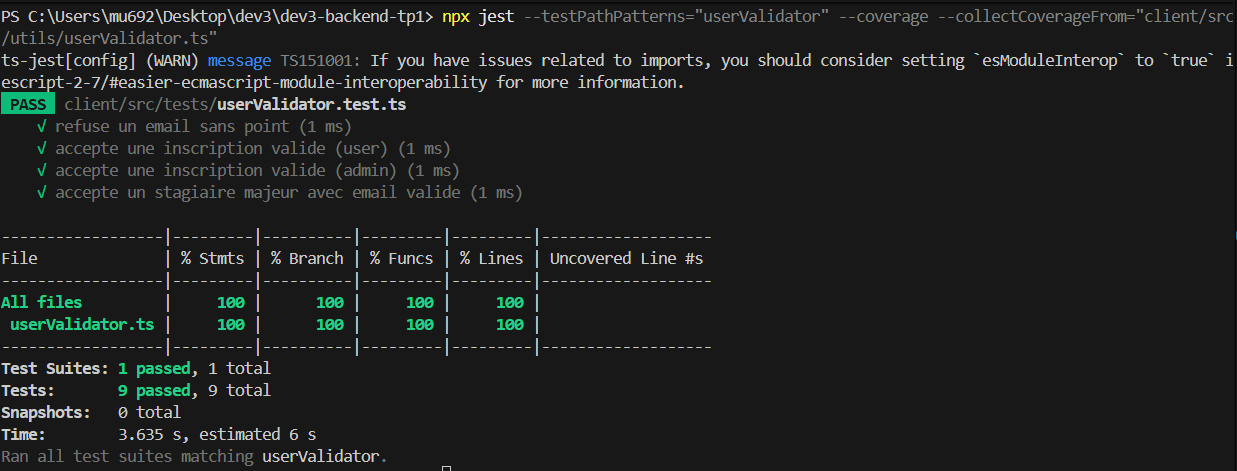
\includegraphics[width=0.9\textwidth]{screenshots/screen_tp4.png}
  \caption{Résultats Jest --- 9 tests passés et 100\% de couverture sur \texttt{userValidator.ts}}
  \label{fig:jest-coverage}
\end{figure}

% =========================================================
\section{Conclusion}
% =========================================================

La démarche appliquée a permis de :
\begin{itemize}
  \item Identifier systématiquement les valeurs limites et les cas d'erreur
        grâce au \emph{Catalog-Based Testing}, sans connaître l'implémentation
        au préalable (\emph{Black Box}).
  \item Réduire à \textbf{12 cas de test} une espace de combinaisons potentiellement
        très large grâce à l'approche \emph{Pairwise}.
  \item Atteindre \textbf{100\% de Branch Coverage} avec 9 tests unitaires Jest,
        en s'assurant que chaque branche conditionnelle de la fonction est exercée.
\end{itemize}

\end{document}
